%%%%%%%%%%%%%%%%%%%%%%%%%%%%%%%%%%%%%%%%%
% baposter Portrait Poster
% LaTeX Template
% Version 1.0 (15/5/13)
%
% Created by:
% Brian Amberg (baposter@brian-amberg.de)
% 
% Modified by: Joseph V. Casillas (jvcasill@email.arizona.edu)
% using UA colors and AAPL lab logo
% 
% This template has been downloaded from:
% http://www.LaTeXTemplates.com
%
% License:
% CC BY-NC-SA 3.0 (http://creativecommons.org/licenses/by-nc-sa/3.0/)
%
%%%%%%%%%%%%%%%%%%%%%%%%%%%%%%%%%%%%%%%%%




%----------------------------------------------------------------------------------------
%	PACKAGES AND OTHER DOCUMENT CONFIGURATIONS
%----------------------------------------------------------------------------------------

\documentclass[a0paper,portrait,columns=2]{baposter}

\usepackage[font=small,labelfont=bf]{caption} % Required for specifying captions to tables and figures
\usepackage{booktabs} % Horizontal rules in tables
\usepackage{relsize} % Used for making text smaller in some places
\usepackage{tipa}
\usepackage{pifont}
\newcommand{\cmark}{\ding{51}}%
\newcommand{\xmark}{\ding{55}}%
\usepackage{amssymb}
\usepackage{multirow}
\usepackage{multicol}
\usepackage{tikz}
\usepackage[margin=.7cm]{caption}
\usepackage{hhline}
\usepackage{colortbl}


\usetikzlibrary{arrows,decorations.pathmorphing,backgrounds,positioning,fit,matrix,trees,mindmap,shapes}

\graphicspath{{figures/}} % Directory in which figures are stored

% UA colors
% UA red	RGB 171   5 32
% UA blue	RGB   0  33 71
% UA copper	RGB 163	102	77

\definecolor{bordercol}{RGB}{0,33,71} % Border color of content boxes
\definecolor{headercol1}{RGB}{171,5,32} % Background color for the header in the content boxes (left side)
\definecolor{headercol2}{RGB}{171,5,32} % Background color for the header in the content boxes (right side)
\definecolor{headerfontcol}{RGB}{255,255,255} % Text color for the header text in the content boxes
\definecolor{boxcolor}{RGB}{255,255,255} % Background color for the content in the content boxes
\definecolor{uared}{RGB}{204,0,51}
\definecolor{uablue}{RGB}{12,35,75}

\usepackage{enumitem}
\setlist{nolistsep}



\begin{document}


\background{ % Set the background to an image (background.pdf)
\begin{tikzpicture}[remember picture,overlay]
\draw (current page.north west)+(-2em,2em) node[anchor=north west]
{
\includegraphics[height=1.1\textheight]{bg}};
\end{tikzpicture}
}

\begin{poster}{
grid=false,
borderColor=bordercol, % Border color of content boxes
headerColorOne=headercol1, % Background color for the header in the content boxes (left side)
headerColorTwo=headercol2, % Background color for the header in the content boxes (right side)
headerFontColor=headerfontcol, % Text color for the header text in the content boxes
boxColorOne=boxcolor, % Background color for the content in the content boxes
headershape=roundedright, % Specify the rounded corner in the content box headers
headerfont=\Large\sf\bf, % Font modifiers for the text in the content box headers
textborder=rectangle,
background=user,
headerborder=closed, % Change to closed for a line under the content box headers
boxshade=plain
}
{}
%
%----------------------------------------------------------------------------------------
%	TITLE AND AUTHOR NAME 
%----------------------------------------------------------------------------------------
%
{\sf\bf \LARGE{Acoustics of Spanish and English coronal stops}}
{\vspace{.6em} \textbf{Joseph V. Casillas}, \textbf{Yamile D\'iaz}, \textbf{Miquel Simonet}\\ 
\smaller{University of Arizona \\ Tucson, Arizona} \\
{\hspace{-7in}
\includegraphics[scale=0.2]{UA_logo}\phantom{.}} \\
{\vspace{-.4in}\smaller \{jvcasill, ydiaz44, simonet\}@email.arizona.edu} \\
{\vspace{-.45in}\phantom{.}\hspace{7in}
\includegraphics[scale=0.35]{aalp_logo}}\vspace{-.6in}}




%----------------------------------------------------------------------------------------
%	INTRODUCTION
%----------------------------------------------------------------------------------------

\headerbox{Introduction}{name=introduction,column=0,row=.05}{

\vspace{.1in}

\textbf{Coronal stops (VOT)}

\vspace{.05in}

\begin{itemize} 
	\item English and Spanish contrast \emph{fortis} with \emph{lenis} stops
	\item One acoustic correlate of contrast is VOT
\end{itemize}

\begin{center}
	\begin{tabular}{@{}cccc@{}}
	\hline 
	        & Lead            & Short-lag       & Long-lag \\ 
	\hline 
	Spanish & \textipa{d}     & \cellcolor{gray!15}\textipa{t} & \\ 
	English &                 & \cellcolor{gray!15}\textipa{d} & \textipa{t} \\ 
	\hline
	\end{tabular}
\end{center}

\begin{itemize}
	\item English uses [spread glottis] while Spanish uses [voice] \cite{beckman2011rate}
\end{itemize}

\begin{center}
	\begin{tabular}{@{}lcc@{}}
	\hline
	Spanish         & \phantom{....}[voice]\phantom{....} & \\
	English         &         & [spread glottis] \\
	\hline
	\end{tabular}
\end{center}

\vspace{.1in}
\textbf{Place of articulation}
\vspace{.05in}

\begin{itemize} 
	\item Spanish /d/ and /t/ are ``dental''
	\item English /d/ and /t/ are ``alveolar''
\end{itemize}

\vspace{.1in}
\textbf{Research questions}
\vspace{.05in}

\begin{itemize}
	\item What are the acoustic correlates of place in coronal stops?
	\item Can we measure the acoustics of the articulatory difference?
	\item How are short-lag stops manifested acoustically?\\ \vspace{-.1in}
	\begin{itemize}
		\item Question not addressed for Spanish \emph{vs.} English
		\item Coronal stop acoustics studied for French \emph{vs.} English \cite{sundara2005acoustic}
	\end{itemize}
\end{itemize}



\vspace{.1in}
\textbf{Goal of present study}
\vspace{.05in}
	\begin{itemize}
		\item[] Provide acoustic measurements of Spanish and English coronal \\ stops to investigate further questions regarding these stops \\ in different populations (bilinguals)
	\end{itemize}

\vspace{.01in}

}


%----------------------------------------------------------------------------------------
%	MATERIALS AND METHODS
%----------------------------------------------------------------------------------------

\headerbox{Method}{name=methods,column=0,below=introduction}{

\vspace{.1in}
\textbf{Materials}
\vspace{.05in}
\begin{itemize}
	\item Consonants in utterance-initial position
	\item \textbf{Consonant} (/d t/) $\times$ \textbf{Language} (English, Spanish) \\ $\times$ \textbf{Stress} (stressed, unstressed) \textipa{[\textprimstress $\sigma$.$\sigma$] vs. [$\sigma$.\textprimstress$\sigma$]}:
	\item 6 (items) $\times$ 2 (consonants) $\times$ 2 (stress) = 24 words
\end{itemize}

\vspace{.1in}
\textbf{Speakers} (N = 14) 
% \vspace{-.05in}
\begin{center}
	\begin{tabular}{@{}lll@{}}
	\hline
	Language & Origin & N \\
	\hline
	Spanish  & Majorca, Spain &  8 \\
	English  & Arizona, US &  8 \\
	\hline
	\end{tabular}
\end{center}

\textbf{Procedure}
\vspace{.05in}
	\begin{itemize}
		\item Auditory stimuli: 6 `talkers' (3 Eng., 3 Sp.) each word produced \\ 3 times. 24 words $\times$ 3 iterations $\times$ 2 languages = 144 stimuli
		\item `Talkers' are male, experiment participants are female
		\item Delayed repetition: ``\_ is the word'' or ``\_ es la palabra''
	\end{itemize}

\vspace{.1in}
\textbf{Acoustics}
\vspace{.05in}
\begin{itemize}
	\item 144 (observations) $\times$ 14 (participants) = 2016 tokens
	\item Acoustic metrics (VOT, Relative intensity, Spectral moments)
\end{itemize}

\begin{center}
	\begin{tabular}{@{}lll}
	\hline
	VOT & Relative intensity & Center of gravity \\
	Standard deviation & Skewness & Kurtosis \\
	\hline
	\multicolumn{3}{@{}l}{{\scriptsize{Note: Spectrum of burst (20 ms Gaussian window left-aligned)}}}\\
\end{tabular}
\end{center}

\textbf{Statistics}
\vspace{.05in} 

\begin{itemize}
	\item Spectral moments and relative intensity regressed on VOT
	\begin{enumerate}
		\item Residuals used as criterion in factorial analysis
		\item Residuals used as predictors in logistic regression
	\end{enumerate}
\end{itemize}


\vspace{.25in}

}






%----------------------------------------------------------------------------------------
%	RESULTS
%----------------------------------------------------------------------------------------

\headerbox{Results}{name=results,column=1,row=.05}{ % To reduce this block to 1 column width, remove 'span=2'

\vspace{.1in}

% \hspace{.2in}\textbf{Factorial analysis of spectral moments and mean intensity}
% \vspace{-.1in}
% \begin{center}
% 	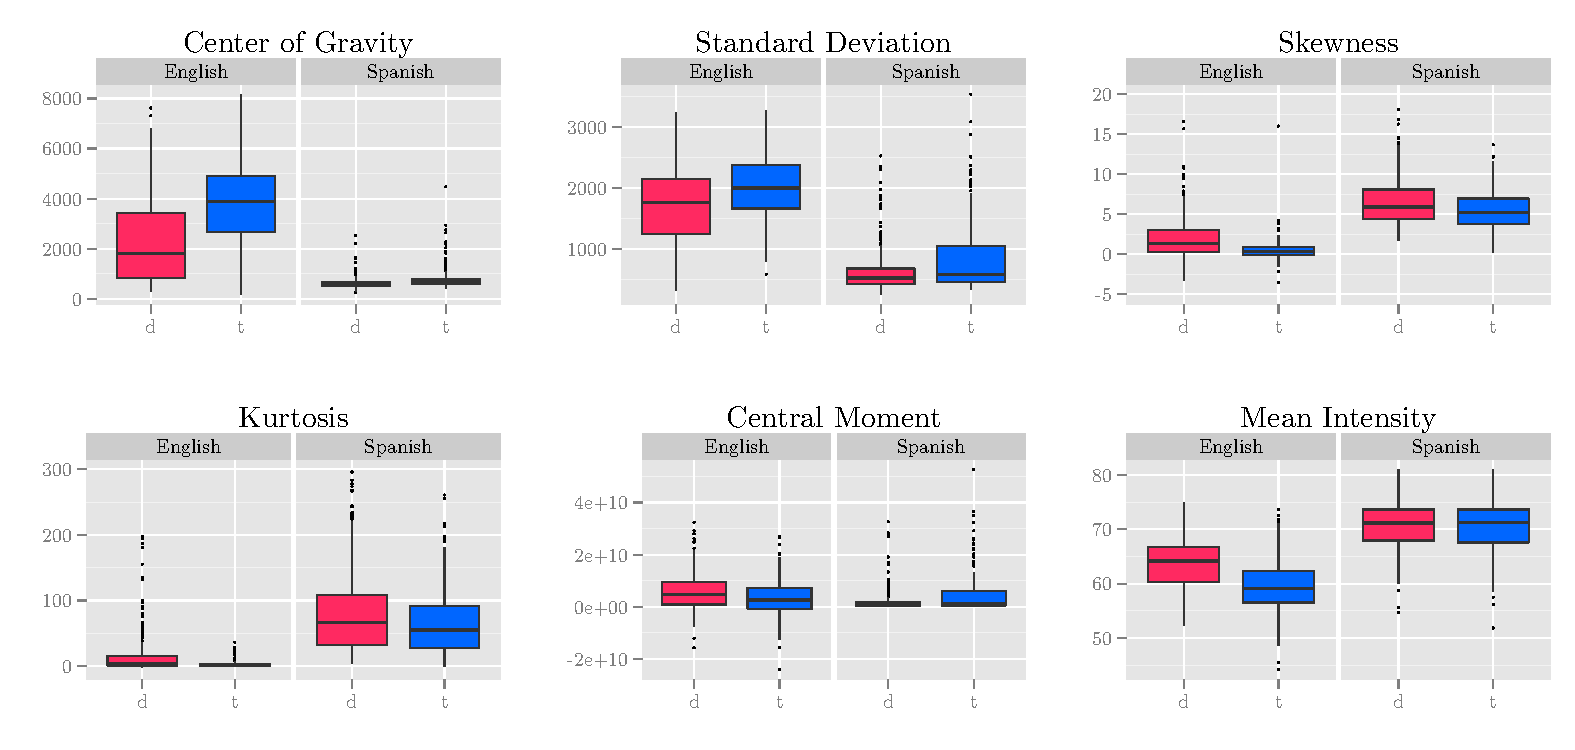
\includegraphics[width=\textwidth]{figures/all.pdf}
% 	\vspace{-.3in}
% 	% Mixed design ANOVA: 1 between subjects factor and 1 withing subjects factor


{\footnotesize{\begin{tabular}{@{}lcccccc}
\hline \\[-2ex]
ANOVA       & COG        & SD  & Skewness   & Kurtosis   & CM  & Mean Intensity \\ [.5ex]
\hline \\[-2ex]
Language &\cellcolor{gray!15} \checkmark &\cellcolor{gray!15} \checkmark &\cellcolor{gray!15} \checkmark & \cellcolor{gray!15} \checkmark & \cellcolor{gray!15} & \cellcolor{gray!15} \checkmark \\ [.5ex]
Voicing      & \checkmark & \checkmark         & \checkmark & \checkmark &                & \checkmark \\ [.5ex]
L $\times$ V & \cellcolor{gray!15} \checkmark & \cellcolor{gray!15} & \cellcolor{gray!15} & \cellcolor{gray!15} & \cellcolor{gray!15} \checkmark & \cellcolor{gray!15} \checkmark \\ [.5ex]
\hline
\multicolumn{7}{@{}l}{{\scriptsize{{DV $\sim$ Language (Spanish, English) $\times$ Voicing (/d t/)}}}}
\end{tabular}
}}


% \end{center}

% \vspace{.2in}

\hspace{.2in}\textbf{\textcolor{uared}{1. Residuals used as criterion in factorial analysis}}
% \vspace{-.05in}
\begin{center}
	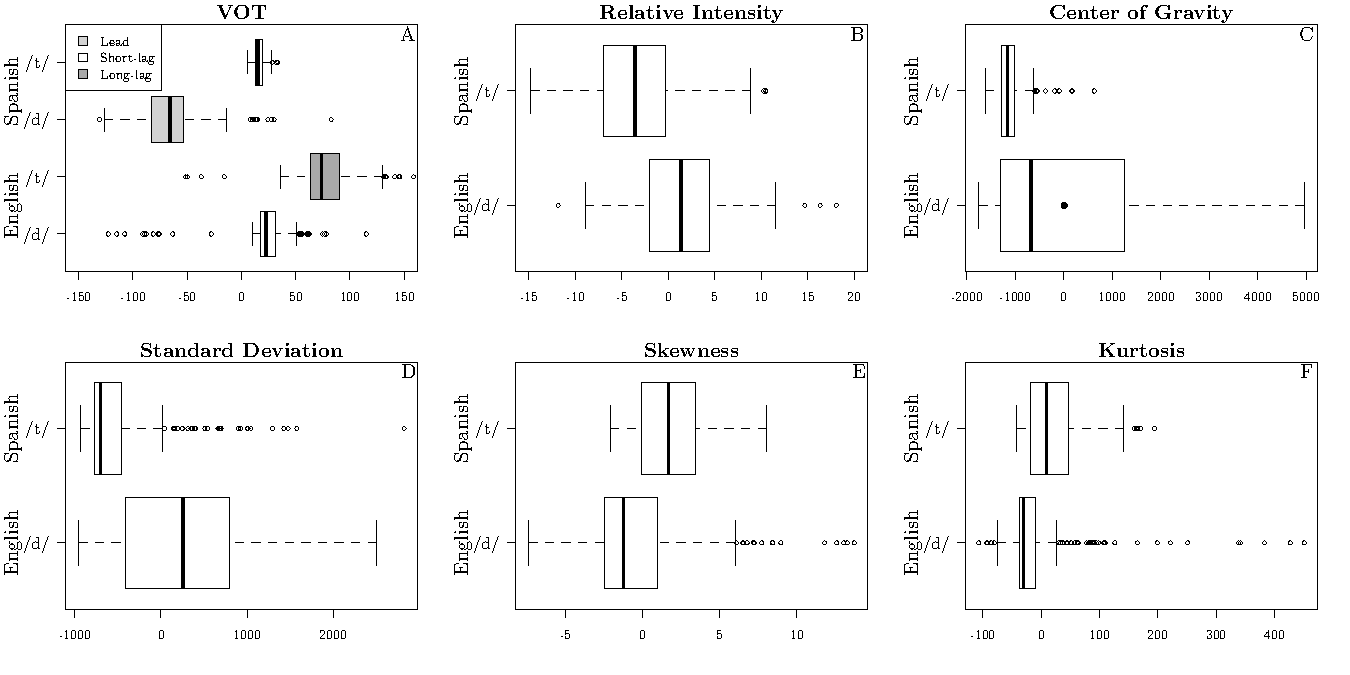
\includegraphics[width=\linewidth]{figures/prod.pdf}
	\vspace{-.2in}
	% Mixed design ANOVA: 1 between subjects factor and 1 withing subjects factor
% uses residuals of linear model as IVs

% {\footnotesize{\begin{tabular}{@{}lcccccc}
% \hline \\[-2ex]
% ANOVA       & COG        & SD         & Skewness   & Kurtosis & CM         & Mean Intensity \\ [.5ex]
% \hline \\[-2ex]
% Language     & \cellcolor{gray!15} & \cellcolor{gray!15} \checkmark & \cellcolor{gray!15} \checkmark & \cellcolor{gray!15} & \cellcolor{gray!15} & \cellcolor{gray!15} \\ [.5ex]
% Voicing      & \checkmark & \checkmark & \checkmark &          &            & \checkmark     \\ [.5ex]
% L $\times$ V & \cellcolor{gray!15} \checkmark & \cellcolor{gray!15} & \cellcolor{gray!15} & \cellcolor{gray!15} & \cellcolor{gray!15}\checkmark & \cellcolor{gray!15}\checkmark \\ [.5ex]
% \hline
% \multicolumn{7}{@{}l}{{\scriptsize{{resid(DV) $\sim$ Language (Spanish, English) $\times$ Voicing (/d t/)}}}}
% \end{tabular}}}

% {\footnotesize{\begin{tabular}{@{}lccccc}
% \hline \\[-2ex]
%          & Relative Intensity & COG & SD & Skewness   & Kurtosis            \\ [.5ex]
% \hline \\[-2.5ex]
% \emph{p-value}  &                    &     &    & \checkmark &                     \\ [.5ex]
% \emph{R}$^2$    &                    &     &    &            &                     \\ [.5ex]
% \hline \\[-2ex]
% \multicolumn{6}{@{}l}{{\scriptsize{{resid(DV) $\sim$ Short-lag stop (Spanish /t/, English /d/) }}}}
% \end{tabular}}}

{\footnotesize{\begin{tabular}{@{}llrr@{}}
\hline \\[-2ex]
Metric             & & \emph{R}$^2$ & \emph{p-value} \\ [.5ex]
\hline \\[-2ex]
Relative Intensity & & 0.66         & < 0.02 \\
Center of Gravity  & & 0.68         & < 0.03 \\
Standard Deviation & & 0.61         & < 0.01 \\
Skewness           & & 0.45         & < 0.03 \\
Kurtosis           & & 0.26         & = 0.07 \\
\hline \\[-2ex]
\multicolumn{4}{@{}l@{}}{{\scriptsize{resid(DV) $\sim$ Short-lag stop (Spanish /t/, English /d/)}}}
\end{tabular}}}



\end{center}

\vspace{.1in}

\hspace{.2in}\textbf{\textcolor{uared}{2. Residuals used as predictors in logistic regression}}\\

\vspace{-.1in}

\hspace{.35in} \scriptsize{Data subset = short-lag VOT stops (Spanish /t/, English /d/)} \\

\begin{center}
	\vspace{-.3in}
	% R2 from logistic regression

{\footnotesize{
	\begin{tabular}{@{}lccccc@{}}
		\hline \\ [-2ex]
		      & COG & Mean Intensity & SD & Skewness & Central Moment \\[.5ex]
		\hline \\ [-2ex]
		R$^2$ & .67 & .54            & .51 & .47     & .0             \\[.5ex]
		\hline
		\multicolumn{6}{@{}l}{{\scriptsize{Consonant $\sim$ \{COG, Mean intensity, SD, Skewness, Central moment\}}}}
	\end{tabular}
}}
\end{center}


\vspace{-.25pt}

%------------------------------------------------


}

%----------------------------------------------------------------------------------------
%	CONCLUSION
%----------------------------------------------------------------------------------------

\headerbox{Conclusion}{name=conclusion,column=1,below=results}{

\vspace{.1in}

\begin{itemize}
	\item VOT accounts for differences between all coronal stops except \\ for English /d/ and Spanish /t/.
	\begin{itemize}
		\item English /d/ and Spanish /t/ do not differ in VOT.
	\end{itemize}
	\item Phonetically voiceless coronal stops of English and Spanish \\ can be distinguished by relative intensity and by 
	the spectral \\ shape of the stop burst.
	\item With regard to the spectral shape of stop burts, place of \\ articulation differences described for Spanish /t/ and \\ English /d/ are best accounted for using measures of \\ standard deviation and center of gravity.
\end{itemize}

\vspace{-.1in}
	\begin{center}
	\begin{tabular}{cl}
	\cmark & Center of Gravity, Standard Deviation \\
	\xmark          & Skewness, Kurtosis \\
	\end{tabular}
	\end{center}
\vspace{-.1in}

\begin{itemize}
	\item Present study contributes language-specific acoustic \\ characteristics of bursts in the short-lag coronal 
	stops in two \\ monolingual varieties of English and Spanish. 
	\item It provides base acoustic descriptions for future studies on \\ Spanish-English bilinguals.
\end{itemize}

\vspace{.1in}
}

%----------------------------------------------------------------------------------------



%----------------------------------------------------------------------------------------
%	REFERENCES
%----------------------------------------------------------------------------------------

\headerbox{Selected references}{name=references,column=1,below=conclusion}{
{\footnotesize
\smaller % Reduce the font size in this block
\renewcommand{\section}[2]{\vskip 0.05em} % Get rid of the default "References" section title
% \nocite{*} % Insert publications even if they are not cited in the poster

\bibliographystyle{unsrt}
\bibliography{IEEEabrv,vot} % Use sample.bib as the bibliography file
\vspace{.02in}
}
}






\end{poster}

\end{document}